\chapter[Molten Salt Reactors]{Molten Salt Reactors}


\section{History}
Developing of \glspl{MSR} started in the late 1940's as part of the United States' program to design a nuclear powered airplane. Particularly  liquid fuel appeared to offer number of advantages, and experiments to demonstrate the feasibility of molten salt fuels were begun in 1947 on ``the initiative of V.P.Calkins, Kermit Anderson, and E.S.Bettis. At the enthusiastic urging of Bettis and on the recommendation of W.R.Grimes, R.C.Briant adopted molten fluoride salts in 1950 as the main line effort of the \glsfirst{ORNL}'s Aircraft Nuclear Propulsion program." The flourides appeared exceptionally suitable because they have high solubility for uranium, are among the most stable of chemical compounds, have low vapor pressure even at temperature more than 1300$^{\circ}$C, have fairly good hydraulic and thermal properties, do not react furiously with air of water, are not damaged by hight neutron fluxes, and are inert to some common structural materials \cite{rosenthal_molten-salt_1970}.

A small test reactor, the \gls{ARE}, was built at Oak Ridge site to probe the use of molten flouride fuels for aircraft propulsion reactors and to study the nuclear stability of the circulating fuel system. Fuel salt for the \gls{ARE} was a mixture of NaF, ZrF$_4$, and UF$_4$, BeO served as moderator, and all the piping was nickel-chromium alloy Inconel. The experiment was successful: in 1954 the \gls{ARE} was operated for 9 days at steady-state outlet temperatures up to 860$^{\circ}$C and at powers up to 2.5 MW$_{(th)}$. No mechanical or chemical problems were observed, and the reactor was found to be stable and self-regulating.

Great potential of \glspl{MSR} for civilian power application was recognized from the beginning of Aircraft Nuclear Propulsion program, and in 1956 H.G.MacPherson founded a group to study the technical characteristics, nuclear performance, and economics of molten salt converting and breeding reactors. After few years of research with number of concepts, MacPherson and his colleagues concluded that graphite-moderated thermal reactors operating on a thorium fuel cycle would be the best choice for applying molten salt systems for producing economic energy. Breeding $^{233}$U from $^{232}$Th was found to give better performance in a molten salt thermal reactor neutron energy spectrum than a uranium fuel cycle in which depleted uranium ($^{238}$U) is the fertile material and fissile $^{239}$Pu is produced and recycled. Homogeneous reactor designs that have entire core consist of liquid sal were rejected because the limited moderation by the salt components did not prove to make good thermal reactor comparing with one moderated by graphite. Furthermore, intermediate spectrum reactors did not appear to have high enough breeding ratios to compensate for their higher inventory of fuel. Later studies of fast spectrum molten salt reactors \cite{kasten_mosel_1964} has shown that effective breeding could be obtained with extremely high power densities that needed to avoid excessive fissile inventories. Acceptable  power densities appeared challenging to achieve without using novel and untested heat transfer technologies.

Two types of graphite-moderated reactors were selected by MacPherson's group for further research: single-fluid reactors in which thorium and uranium are dissolved in the same carrier salt, and two-fluid design in which a fertile salt accommodated $^{232}$Th is separated from the fissile salt which contains $^{233}$U and/or $^{239}$Pu as initial fissile load for reactor startup. The two-fluid reactor could operates as breeder but construction materials separating flows would significantly deteriorate neutron economy and, consequently, breeding ratio. The single-fluid design is much simplier, easier to build and offers lower power costs, even for that time technology which could only achive breeding ratio slightly below 1.0. The chemical reprocessing method namely fluoride volatility process, which separates uranium from flouride salts, had been already demonstrated during \gls{ARE} for recovery uranium from \gls{ARE} fuel salt and might be used for partial reprocessing of salts from another type of reactor.

U.S. Atomic Energy Commission task force have considered results of the \gls{ORNL} research and made a comparative evaluation of fluid-fueled reactors early in 1959. One conclusion of the task force was that the \gls{MSR} even limited in potential breeding gain, had ``the highest probability of achieving technical feasibility." \cite{noauthor_report_1959}

In 1960s more complete conceptual \gls{MSR} designs have been developed. \gls{ORNL} conculed that both single-fluid and two-fluid concepts whould lead to low-power-cost reactors, and that progressing to the breeder either directly or using the converter would create reactors with good fuel utilization characteristics \cite{rosenthal_molten-salt_1970}. Because of many of the features of commercial power reactors would differ from those for the \gls{ARE}, and the \gls{ARE} had beed operated only a short period of time, new reactor experiment with molten salt was necessary to investigate some of the technology for civilian power reactors.

The developing of the \gls{MSRE} was started in 1960. Creators selected a single-fluid design because it is similar to a converter, but the fuel salt did not contain thorium, consequently, was similar to the fuel salt composition for a two-fluid breeder. The \gls{MSRE} fuel salt is a mixture of uranium, $^7$Li, beryllium, and sirconium fluorides. Bare graphite serves as the moderator because the salt cannot penetrate into its pores if the pore sizes are small. Specially developed in the aircraft program nickel-based alloy INOR-8 (also called Hastelloy-N) for use with molten fluorides was employed as a main constuction material for piping and other elements of the system. The maximum power is about 8MW$_{th}$, and the heat is dissipated to the atmosphere \cite{haubenreich_experience_1970}.

Construction of the \gls{MSRE} has begun in 1962, and the reactor first became critical in 1965. Figure~\ref{fig:msre} has shown graphite reactor core assembling. Continuous operation at full power level began in December 1966. Successful completion of a six-month test campaign in March of 1968 closed the first phase of operation, all initial objectives were achived. The molten fluoride fuel salt was used in the reactor core for many month at temperatures $\geq$649$^{\circ}$C without corrosive damaging of the metal and graphite elements of the system. All reactor equipment worked reliably, radioactive liquids and gases were holded safely, te fuel salt was absolutely stable. Xenon was removed continuously from the salt. Radiactive components was reapaired or replaced in acceptable time without overexposing mainenance personnel.

The second stage of \gls{MSRE} has started in August 1968 when a small chemical processing facility connected with the reactor was used to remove the original uranium from the fuel salt using fluorine gas. $^{233}$U fuel was added to the same carrier salt, and on October 2 the \gls{MSRE} begun operation on $^{233}$U. Six days later the power was achieved 100 kW by Glenn T.Seaborg, Chairman of the U.S. Atomic Energy Commission, bringing to power the first in a world reactor operating on $^{233}$U \cite{haubenreich_experience_1970}.

\begin{figure}[htp!] % replace 't' with 'b' to 
  \centering
  \vspace{-0.3em}
  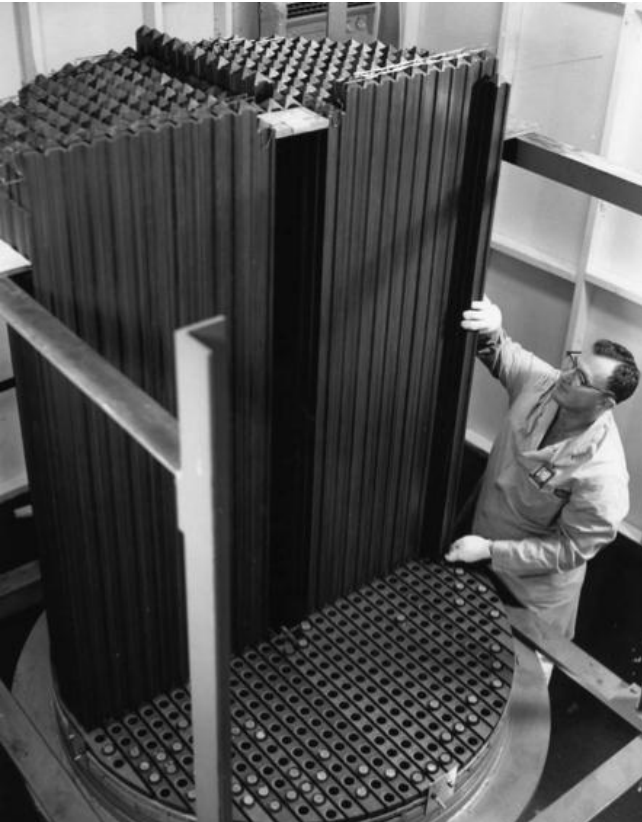
\includegraphics[width=0.75\textwidth]{msre_view.png}
  \caption{The \gls{MSRE} core, shown while being assembled, contains about 1.95 m$^3$ of reactor graphite. The 1140 fuel channels contain about 0.57m$^3$ of fuel salt.}
  \vspace{-0.6em}
  \label{fig:msre}
\end{figure}
\FloatBarrier

After \gls{MSRE} was build and brought into operation, most of the research and development work on \glspl{MSR} was in support of the \gls{MSRE}. However, molten fluoride salts chemistry keep developing during this period, i.e. was discovered method of separation lithium fluoride and beryllium fluoride from rare earths by vacuum distillation at temperature about 1000$^{\circ}$C. This method provided an inexpensive, on-site way for recovering valuable rare materials, following this, the study effort for future reactors changed focus to a two-fluid breeder. In this reactor the fuel salt should be fluorinated to recover the uranium and distilled to separate carrier salt from fission products. The blanket salt would be reprocessed by just fluorination because only few fission products might be generated in the blanket if the fissile material concentration were kept low and no fission happens in the blanket. Graphite tubes in the core were designed to prevent the fuel and fertile streams from mixing.

Two-fluid systems analysis have shown that breeding ratio could be about 1.07, which with low fissile inventory would lead to relatively good fuel utilization. Therefore, the development effort for future reactors was concentrated at the futures of two-fluid breeders. The main drawback of those reactors was identified as graphite pipes damaging by very high neutron fluxes.

Later, in 1967, new experimental information obtained from \gls{MSRE} and an advance in core design lead to change \gls{ORNL} molten salt program R\&D focus from the two-fluid to a single-fluid breeder. This switch was based on concerns about graphite behavior at higher radiation exposures that had been achieved previously, graphite changes dimensions more rapidly than had been acticipated. To use that kind of graphite in \gls{MSBR} it was necessary to lower the core power density to achieve acceptable graphite lifetime, and to plan on replacement of the core at realistically frequent intervals. Furthermore, complexities in the assembly of the core required the entire core and reactor vessel replacement when any graphite element reached its irradiation limit or developed a leak \cite{rosenthal_molten-salt_1970}.

Because of problems associated with long graphite exposure and significant development of chemical processing \gls{ORNL} decided to change focus to single-fluid breeder.To achieve acceptable breeding ratio in single-fluid reactor, $^{233}$Pa (27.4-day half-life) must be separated from the fuel salt and held up outside the core until it decays to $^{233}$U. Laboratory experiments demonstrated liquid-liquid extraction process for removing protactinium and uranium from molte fluoride salts. The method is to exchange throium and lithium dissolved in molten bismuth for the components to be removed from the salt.Additional data have confirmed that the uraniuum can be selectively separted from the salt, the protctinium can be trapped in the salt in a decay tank, and the uranium can be returned back to the fuel salt by electrolysis for the further transfer to the core. Analysis indicated that the extraction and electrolysis could be carried out rapidly and continuously.

The fertile ``blanket'' in the single-fluid breeder is obtained by increasing the volume fraction of fuel salt and reducing the volume fraction of graphite in the outer part of the reactor. This advanced core design makes the outer region undermoderated and increases neutron capture there by the thorium. Moreover, most of neutrons are born at some distance from the reactor boundary, and captures in outer region reduce the neutron leakage. Further studies indicated that the fuel utilization in single-fluid, two-region \gls{MSR} can be as good as in two-fluid prototype, and even with the limitation on graphite lifetim the economics might be better. Thus, in 1968 \gls{ORNL} \gls{MSR} Program was oriented toward the development of single-fluid breeder reactor.

Despite the success of \gls{ARE} and \gls{MSRE}, the \gls{MSR} program closed down in the early 1970s in favor of the liquid metal fast-breeder reactor (LMFBR),\cite{macpherson_molten_1985} after which research stagnated in the United States. As of 2018, the \gls{ARE} and \gls{MSRE} remained the only molten-salt reactors ever operated.

Recently, interest in \glspl{MSR} has resurged, with multiple new companies pursuing commercialization of \gls{MSR} designs\footnote{Examples include both liquid-fueled molten salt designs from Transatomic, Terrapower, Terrestrial, and Thorcon.}. China initiated a thorium molten salt reactor research project, demonstration of the liquid fuel version (TMSR-LF) are targeted for 2024. European Union funding Safety Assessment of the Molten Salt Fast Reactor (SAMOFAR), in which several European research institutes and universities developing various molten salt reactor prototypes such as \gls{MSFR}, \gls{MOSART}, \gls{FHR}.
To further develop these \gls{MSR} concepts, particularly with respect to their strategies for online reprocessing and refueling, computational analysis methods capturing their unique reactor physics and process chemistry are needed.

\section{Thorium fuel cycle overview}
In the early days of nuclear energy industry, in the United States as a follow-up of the Manhattan Project (1945-1960), US national laboratories studied thorium as a possible substitute for uranium and the possibilty of using $^{233}$U in a nuclear weapon. In the Atoms for Peace Program, with its great variety of developments (1955-1975), thorium appeared to be an interesting resource for supplementing limited uranium availability in the context of a fast-growing nuclear industry because thorium is  at least 4-5 times more abundant than uranium in Earth’s crust and preparation of thorium fuel does not require difficult and expensive enrichment processes. International Fuel Cycle Evaluation Conference (INFCE) of 1978 predicted equal thorium almost equal importance as uranium. It stated that in case of the optimistic nuclear energy development scenario, thorium was to be called upon massively in the future. These predictions were too optimistic, but in a long-term, the use of thorium along with uranium could significantly improve the potential of nuclear energy \cite{lung_perspectives_1998}.

During this pioneer period, the thorium fuel cycle study and developng pre-industrial demonstration reactors were initiated, first in the United States under cooperation between the USAEC and US industry, then in Europe.
About 1500 kg of $^{233}$U have been separated in the United States from 900 tonnes of thorium. Many reactor prototypes as well as thorium extraction plants were built and operated in many countries. The U.S. and France have each separated about 2000 metric tons of thorium, part of which is still available \cite{lung_perspectives_1998}. However, for most countries uranium was relatively abundant and research in thorium fuel cycles diminished. A notable exception was India's three-stage nuclear power program \cite{natarajan_fast_2007}. In the twenty-first century thorium's potential for improving proliferation resistance and waste characteristics couses renewed interest in the thorium fuel cycle \cite{bagla_thorium_2015}.

Comparing with natural uranium which contains 99.284\% $^{238}$U, thorium almost exclusively composed of $^{232}$Th. It can be seen from figure~\ref{fig:th_cycle} that the fertile isotopes are $^{238}$U and $^{232}$Th and that the fissile isotopes are $^{235}$U, 0.711\% of natural uranium present in nature, and the artificial fissile isotopes $^{239}$Pu for uranium and $^{233}$U for thorium. 

In the Uranium-Plutonium cycle production of fissile material ($^{239}$Pu) in a fast-spectrum reactor occurs by neutron irradiation of fertile material ($^{238}$U), while in the thorium fuel cycle $^{232}$Th absorbs a neutron in either a fast or thermal reactor. Next the $^{233}$Th emits an electron and an anti-neutrino by $\beta^-$ decay to become $^{233}$Pa. The protactinium then emits another electron and anti-neutrino by a second $\beta^-$ decay to become $^{233}$U, which in turn is used as fuel. In \glspl{MSR} designs, the $^{233}$Pa is extracted and protected from neutrons (to prevent the core's poisoning and $^{233}$Pa transformation into $^{234}$Pa and then to $^{234}$U), until it has decayed to $^{233}$U. This is done in order to improve the breeding ratio which is low compared to fast reactors. 

\begin{figure}[t] % replace 't' with 'b' to 
  \centering
  \vspace{-0.3em}
  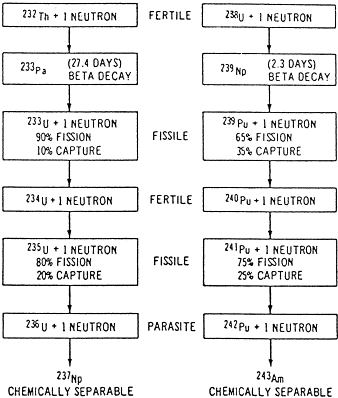
\includegraphics[width=0.70\textwidth]{th_u_cycle.png}
  \caption{Isotopic build-up in $^{232}$Th and $^{238}$U breeding systems \cite{eschbach_possible_1966}.}
  \vspace{-0.6em}
  \label{fig:th_cycle}
\end{figure}
\FloatBarrier

Although the thermal neutron fission cross section $\sigma_f$ of the resulting $^{233}$U is comparable to $^{235}$U and $^{239}$Pu, but has a much lower capture cross section $\sigma_c$ than other two fissile isotopes, providing fewer non-fissile neutron absorptions and improving neutron economy. Figure~\ref{fig:n_yeild} shows the ratio of neutrons released per neutron absorbed $\eta$ which in $^{233}$U is greater than two over a wide range of energies, including the thermal spectrum, consequently, thorium fuels can be the basis for a thermal breeder reactor \cite{iaea_thorium_2005}. A breeding reactor in the U-Pu cycle required a fast neutron spectrum, because in the thermal spectrum one neutron absorbed by $^{239}$Pu in average produces less than two neutrons.

Another advantage of thorium fuel cycle is inherent prolifiration resistance due to contamination of fissile $^{233}$U with $^{232}$U in proposed power reactor designs. $^{232}$U cannot be chemically separated from $^{233}$U and has few decay products that emit high-energy gamma radiation. These high-energy $\gamma$-rays are a radiological hazard, thus, remote handling necessarily for separated uranium and such materials could be easly detected.

\begin{figure}[htbp!] % replace 't' with 'b' to 
  \centering
  \vspace{-0.3em}
  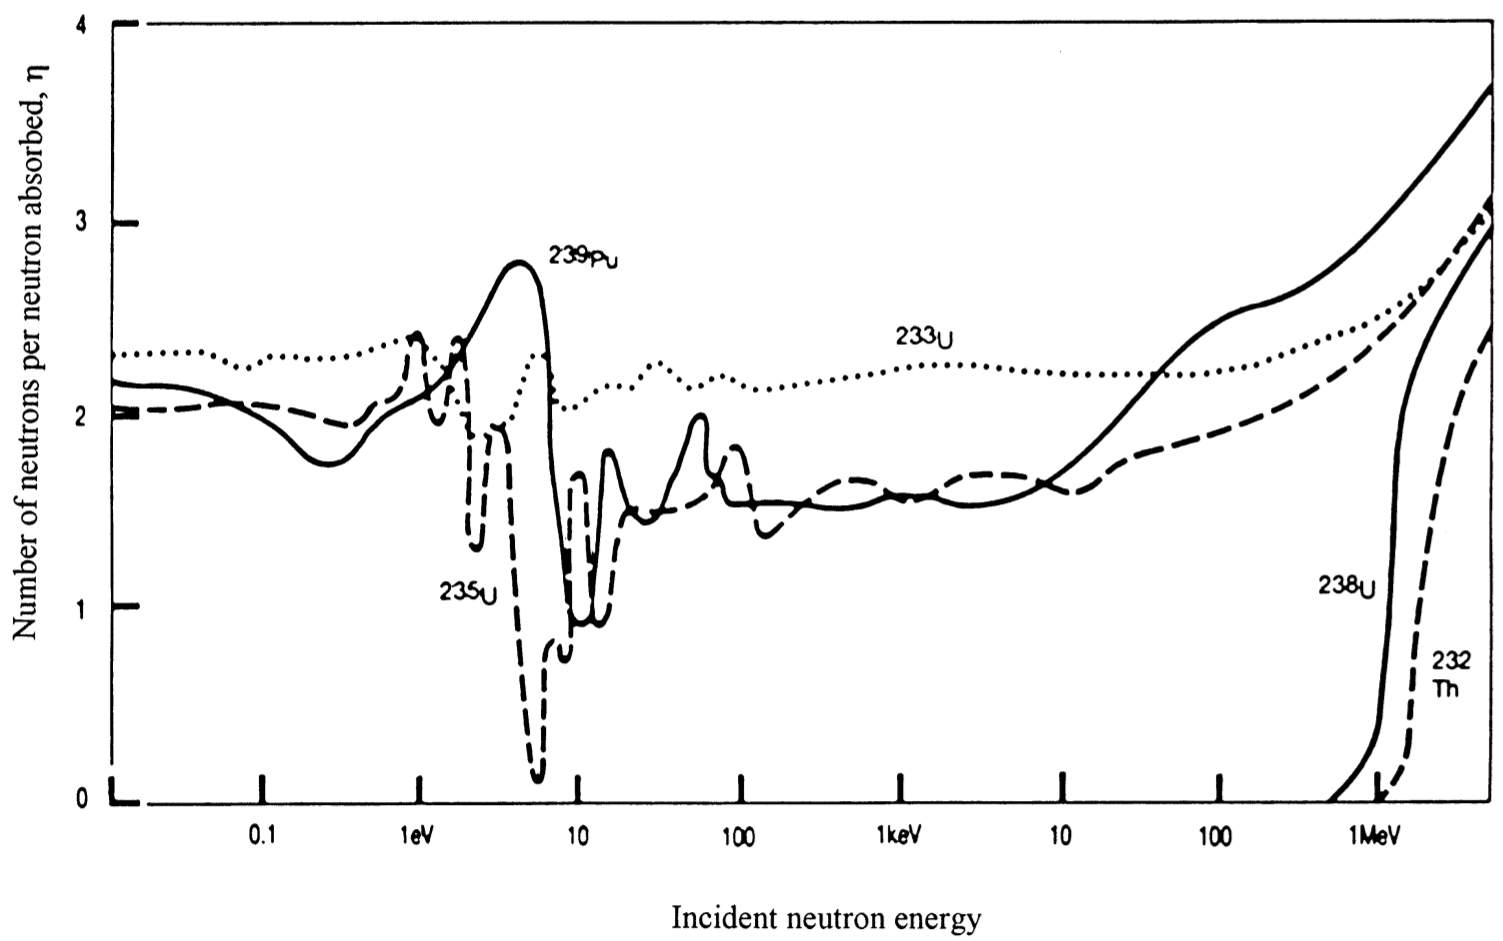
\includegraphics[width=\textwidth]{neutron_yeild.png}
  \caption{Neutron yield per neutron absorbed \cite{anon_plutonium_1989}.}
  \vspace{-0.6em}
  \label{fig:n_yeild}
\end{figure}
\FloatBarrier

Moreover, from the respective positions of uranium and thorium in periodic table, the long-lived minor actinides resulting from fission are in much lower quantity in the thorium cycle, especially compared with the uranium-plutonium cycle. Because of this, thorium is a potentially attractive alternative to uranium in \gls{MOX} fuels to minimize the generation of long-live transuranium elements and maximize the destruction of plutonium.

For the many reasons explained above, thorium fuel cycle is not soo far been able to compete on a par with uranium, which currently occupies a nuclear energy. The
time has come to have another hard look at what was perhaps too quickly set aside forty years ago and restart with new advanced computational methods. 

\section{Literature review}
While most contemporary nuclear reactor physics software is unable to perform depletion calculations in an online reprocessing regime. Furthermore, no established liquid-fueled \gls{MSR} tool for neutronics and fuel cycle evaluation, there are codes from universities, research institutions, and internally developed tools for online refueling approximation \cite{serp_molten_2014}. The foundation for these tools was based on early \gls{MSR} programs  methods at \gls{ORNL}, which integrated neutronic and fuel cycle codes \cite{bauman_rod:_1971} into operational plant tools \cite{kee_mrpp:_1976} for \gls{MSR} and reprocessing system designing. More recent research efforts in Europe and Asia mainly focused on fast spectrum reactors fuel cycle analysis and use some external tools to couple neutron transport and depletion codes to take into account continuous feeds and removals in \glspl{MSR}. Four of these works listed in table~\ref{tab:fs_codes}.

\begin{table}[h!]
\centering
\caption{Tools and methods for fast spectrum system fuel cycle analysis.}
\begin{tabular}{ |m{0.02\textwidth}|m{0.3\textwidth}|m{0.2\textwidth}|m{0.35\textwidth}|} 
\hline
\# & Neutronic code  & Depletion code    & Authors         \\[5pt]
\hline
1 & \gls{MCNP} \cite{noauthor_mcnp_2004}      & REM \cite{heuer_simulation_2010}  & Doligez \emph{et al.}, 2014; Heuer \emph{et al.}, 2014 \cite{doligez_coupled_2014,heuer_towards_2014}    \\[5pt]
\hline
2 & ERANOS \cite{ruggieri_eranos_2006}      & ERANOS     & Fiorina \emph{et al.}, 2013 \cite{fiorina_investigation_2013}\\[5pt]
\hline
3 & KENO-IV \cite{goluoglu_monte_2011}     & ORIGEN \cite{gauld_isotopic_2011}     & Sheu \emph{et al.}, 2013 \cite{sheu_depletion_2013} \\[5pt]
\hline
4 & SERPENT 2 \cite{leppanen_serpent_2015}   & SERPENT 2  & Aufiero \emph{et al.}, 2013 \cite{aufiero_extended_2013} \\[5pt]
\hline
\end{tabular}
  \label{tab:fs_codes}
\end{table}

Most of these methods are applicable to thermal spectrum reactors, moreover, additional tools developed specifically for thermal \gls{MSR} applications listed in table~\ref{tab:th_codes}.

\begin{table}[h!]
\centering
\caption{Tools and approaches for thermal spectrum system fuel cycle analysis.}
\begin{tabular}{ |m{0.02\textwidth}|m{0.2\textwidth}|m{0.2\textwidth}|m{0.45\textwidth}|} 
\hline
\# & Neutronic code  & Depletion code    & Authors         \\[5pt]
\hline
5 & MCODE \cite{xu_mcode_2008}      & ORIGEN2 \cite{croff_users_1980}      & Ahmad \emph{et al.}, 2015 \cite{ahmad_neutronics_2015}     \\[5pt]
\hline
6 & \gls{MCNP}6     & CINDER90 \cite{goorley_mcnp6_2013}     & Park \emph{et al.}, 2015; Jeong \emph{et al.}, 2016 \cite{park_whole_2015, jeong_equilibrium_2016}\\[5pt]
\hline
7 & SCALE \cite{bowman_scale_2011}      & SCALE/ ChemTriton \cite{powers_new_2013}    & Powers \emph{et al.}, 2014; Betzler \emph{et al.}, 2017 \cite{powers_new_2013,powers_inventory_2014,betzler_molten_2017}\\[5pt]
\hline
8 & SERPENT 2      & SERPENT 2     & Rykhlevskii \emph{et al.}, 2017 \cite{rykhlevskii_online_2017} \\[5pt]
\hline
9 & \gls{MCNP}      & REM  & Nuttin \emph{et al.} \cite{nuttin_potential_2005}    \\[5pt]
\hline
\end{tabular}
  \label{tab:th_codes}
\end{table}

Methods (1,3,4) provide some form of reactivity control, and methods (1,4,5,6,8,9) use inventory of all nuclides in depletion calculations. 

Liquid-fueled \gls{MSR} have online separations and/or feeds, where material is moved to or from the core at all times (continuous) or at specific time steps (batch). To account for batch discards, a depletion tool should have capability to remove fraction or all material at specified interval. This requires the burn-up simulation to stop ar a given time and restart with a new liquid fuel composition (after removal of discarded matherials and addition fissile/fertile materials). Accounting for a continuous removal or addition is more difficult because it required adding a term to the Bateman equations. In SCALE \cite{bowman_scale_2011}, ORIGEN \cite{gauld_isotopic_2011} solves a set of Bateman equations using spectrum-averaged fluxes and cross sections generated from transport calculation. Methods (1,4,8) provide opportunity to work with true continuous feeds and removals, while other methods employed batch-wise approach. \gls{ORNL} researchers developed ChemTriton, Python-based script for SCALE/TRITON which uses a semi-continuous batch process to simulate a continuous reprocessing. This tool models salt treatment, separations, discards, and refill using an unit-cell \gls{MSR} SCALE/TRITON model over small time steps to simulate continuous reprocessing and deplete the fuel salt \cite{powers_new_2013}.

Thorium-fueled \gls{MSBR}-like reactors similar to one in this thesis described in (6,7,8,9). Moreover, most of these efforts considered only simplified unit-cell geometry because depletion computations for few year cycle are very computationally expesive even for simple models. 

Nuttin \emph{et al.} broke up reactor core geometry into tree \gls{MCNP} cells: one for salt channels, one for two salt plena above and below the core and the last cell for the annulus, consequently, two-region reactor core was approximated by one region with averaged fuel/moderator ratio \cite{nuttin_potential_2005}.  Similar approach was used by Powers \emph{et al.}, Betzler \emph{et al.}, Jeong \emph{et al.} \cite{powers_new_2013,powers_inventory_2014,betzler_modeling_2016, betzler_molten_2017, jeong_development_2014, jeong_equilibrium_2016} and clearly misrepresent two-region breeder reactor concept. The unit-cell or one-region models may produce reliable results for homogeneous reactor cores (i.e. \gls{MSFR}, \gls{MOSART}) or for one-region single-fluid reactor designs (i.e. \gls{MSRE}). Two-region \gls{MSBR} must be simulated using whole-core model to represent different neutron transport in inner and outer region of the core, because most of fissions happens in inner region while breeding occurs in outer zone.  

Aufiero \emph{et al.} extended Monte Carlo burn-up code SERPENT 2 and employed it to study the material isotopic evolution of the \gls{MSFR}. The developed extension directly takes into account the effects of online fuel reprocessing on depletion calculations and features a reactivity control algorithm. The extended version of SERPENT 2 was assessed against a dedicated version of the deterministic ERANOS-based EQL3D procedure \cite{ruggieri_eranos_2006} and adopted to analyze the \gls{MSFR} fuel salt isotopic evolution. Rykhlevskii \emph{et al.} employed this extended SERPENT 2 for simplified unit-cell geometry of thermal spectrum thorium-fueled \gls{MSBR} and obtain contradictory results with existing \gls{MSBR} depletion simulations \cite{jeong_equilibrium_2016}.

Chapter 2 and 3 of current study most similar to the works described in (6,7,9), but focus is on developing new external open-source tool for online reprocessing simulation named Saltproc. The tool works with Monte Carlo code SERPENT 2, has reactivity control module which allows ajust reactivity by changing feed material flow and avoid control rod movement. Moreover, recent research efforts are being extended by using for online reprocessing simulation high-fidelity full-core 3-D model without any approximations in the core geometry.

Another challenge presented by liquid-fueled systems is the fuel materials movement. Fuel flow is important because of delayed neutron emission. In reactor with solid fuel, the fission product delayed neutron precursors remain very close to the location where fission happened, later emitting delayed neutrons at that location. Delayed neutrons has softer energy spectrum than prompt neutrons. In case of liquid-fuled reactors the precursors drift and the fission and delayed neutron emmition location are different. The reactor design determines the effect of the precursor drift on the core physics. The flow parameters (e.g., flow rate, pipe diameter, primary loop length) affect on the effective delayed neutron fraction ($\beta_{eff}$). This quantity has significant impact on reactor safety because delayed neutron production occurs on a relatively large time frame to allow control a reactor. Hence, to take into account tightly coupled \gls{MSR} neutronics, thermal-hydraulics and the precursors drift multi-physics code required.

There are number of multi-physics tools developed by many authors which successfully describe steady-state and transient behavior of various \gls{MSR} concepts. Krepel \emph{et al.} extended the \gls{LWR} diffusion code DYN3D to consider drift of delayed neutron precursors alongside the reactor temperature profile, re-introducing the extended code as DYN3D-MSR \cite{krepel_dyn3d-msr_2007}. That work compared DYN3D-MSR against experimental \gls{MSRE} data to simulate local fuel channel blockages as well as local temperature perturbations.

Similarly, Kophazi \emph{et al.} used iterative coupling between three-dimensional neutronic and one-dimensional heat conduction models DALTON and THERM to analyze normal \gls{MSRE} operation as well as channel-blocking-incident transients \cite{kophazi_development_2009}. The Kophazi model added entrance effects of heat transfer coefficients as well as thermal coupling between fuel channels through moderator heat conduction. Later, Cammi \emph{et al.} performed a 2D-axisymmetric single-channel analysis of the \gls{MSBR} using the commercial finite element package COMSOL Multiphysics \cite{cammi_multi-physics_2011}. That work directly solved the fuel salt velocity field, used heterogeneous group constants in fuel and moderator regions.  

More recently, Aufiero \emph{et al.} \cite{aufiero_development_2014} have approach to transient simulations in the \gls{MSFR} within the finite volume
OpenFOAM multiphysics toolkit \cite{weller_tensorial_1998}.  This approach
benefits from pre-implemented turbulence models available in the OpenFOAM
library and captures the full-core three-dimensional geometry of the reactor
primary circuit.  OpenFOAM \gls{CFD} has additionally been shown by Laureau et
al. \cite{laureau_transient_2017} to couple well with Transient Fission Matrix
neutronics within the \gls{MSFR}.

Concurrently, Lindsay \emph{et al.} have introduced Moltres, a physics application for multiphysics modeling of liquid-fueled \glspl{MSR} \cite{lindsay_introduction_2018}. It couples equations for neutron diffusion, thermal-hydraulics, and delayed neutron precursor transport. Moltres solves arbitrary-group neutron diffusion, temperature, and precursor governing equations in anywhere from one to three dimensions and can be deployed on an arbitrary number of processing units. That work compared 2D-axisymmetric many-channel anlysis of the \gls{MSRE} in Moltres agains experimental \gls{MSRE} data in steady-state mode.

On the whole, all these research efforts used initial fuel salt composition, consequenly, consider reactor core for at the moment of startup. Chapter 4 of the present thesis introduces the steady-state multi-physics analysis of \gls{MSBR} using Moltres code for both initial fuel composition and for equilibrium fuel composition.

